\documentclass{article}%
\usepackage[T1]{fontenc}%
\usepackage[utf8]{inputenc}%
\usepackage{lmodern}%
\usepackage{textcomp}%
\usepackage{lastpage}%
\usepackage{authblk}%
\usepackage{graphicx}%
%
\title{Preventive effect of caffeine and curcumin on hepato\_ carcinogenesis in diethylnitrosamine\_induced rats}%
\author{Jerry Bautista}%
\affil{Department of Genetics, Washington University School of Medicine, St. Louis, Missouri, United States of America}%
\date{01{-}01{-}2011}%
%
\begin{document}%
\normalsize%
\maketitle%
\section{Abstract}%
\label{sec:Abstract}%
SELECTING THE OPTIONS at the NEAM Learning Center\newline%
COLUMBUS, OH (January 1, 2011) {-} The Carter Centers for Disease Control (CDC) and Prevention (CDC) through National Institutes of Health (NIH) sponsored an educational event for primary care doctors, rheumatologists, allergy specialists, immunologists, immunocontrol specialists, nurse practitioners, and other health care professionals to help them determine the potential benefits and risks of immunizations. Key providers of immunized children in the hearing screening program discussed the benefits and the need for immunization in children and adolescents.\newline%
"The importance of immunization is not defined by age but rather by the variety of preventable diseases that we can address as a family," said William Walters, M.D., M.P.H., director of the MD Anderson Center for Immunization Policy and Clinical Practices at The University of Texas Medical Branch at Galveston (UTMB). "In the United States, several million Americans have been given vaccines at a young age, including 40 million through routine immunizations, and in addition, approximately 10 percent of the U.S. population can be prevented from becoming sick by using the childhood immunization schedule."\newline%
The event presented by the Carter Center in coordination with NIH funded studies concluded that preventive immunization using the cyclo{-}carotid amyloid beta (CD11) antigen as an adjuvant provides protection against a range of ailments and improves outcomes for the newborns and infants in families. The study found that the amyloid beta immunity and the added protection against older, more severe ailments was not that different from that obtained from conventional immunizations and now is worth the cost of the adjuvant that does not require the use of a systemic therapy in the newborn who has a B11 antigen exposure.\newline%
"Infants who receive these preventive vaccines before they are five months of age receive immunity for at least 60 years," explained Albi Larson, M.D., a neonatologist who was part of the study. "Adjuvants could improve the immune system by preventing the cancer{-}causing B12 Epstein{-}Barr virus (EBV) infection and if antibodies to EBV are acquired during the treatment, they could avoid the disease for nearly half a century."\newline%
In addition to the findings of the study, interested participants were able to go to the CD11 adjuvant antibody lab and meet with empathetic providers who can help them understand the implications of the ADIA 2 prevention protocols and how the vaccine may protect against other childhood disorders as well as the health and developmental challenges associated with the late onset of life. Data were also obtained on the immunization therapy in The Dime Quotient Trial of methylnaltrexone (MQT) in hospitalized newborns and mothers of infants who are infected with the disease.\newline%
Other drug factors in the study that included the use of the optional adjuvant may also be discussed in this event.\newline%
"Some of these drug factors have been studied and shown to be associated with adverse side effects in clinical trials, however, I think the vaccine is a safer substitute," said Dr. Larson. "The telemedicine opportunities provided by the CEU is ideal in this setting and includes information and assistance from the healthcare professionals treating children like ours."

%
\subsection{Image Analysis}%
\label{subsec:ImageAnalysis}%


\begin{figure}[h!]%
\centering%
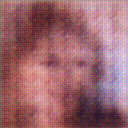
\includegraphics[width=150px]{500_fake_images/samples_5_158.png}%
\caption{A Close Up Of A Black And White Cat}%
\end{figure}

%
\end{document}